%********************************************%
%*       Generated from PreTeXt source      *%
%*       on 2020-08-18T01:28:50-03:00       *%
%*   A recent stable commit (2020-08-09):   *%
%* 98f21740783f166a773df4dc83cab5293ab63a4a *%
%*                                          *%
%*         https://pretextbook.org          *%
%*                                          *%
%********************************************%
\documentclass[oneside,10pt,]{article}
%% Custom Preamble Entries, early (use latex.preamble.early)
%% Default LaTeX packages
%%   1.  always employed (or nearly so) for some purpose, or
%%   2.  a stylewriter may assume their presence
\usepackage{geometry}
%% Some aspects of the preamble are conditional,
%% the LaTeX engine is one such determinant
\usepackage{ifthen}
%% etoolbox has a variety of modern conveniences
\usepackage{etoolbox}
\usepackage{ifxetex,ifluatex}
%% Raster graphics inclusion
\usepackage{graphicx}
%% Color support, xcolor package
%% Always loaded, for: add/delete text, author tools
%% Here, since tcolorbox loads tikz, and tikz loads xcolor
\PassOptionsToPackage{usenames,dvipsnames,svgnames,table}{xcolor}
\usepackage{xcolor}
%% begin: defined colors, via xcolor package, for styling
%% end: defined colors, via xcolor package, for styling
%% Colored boxes, and much more, though mostly styling
%% skins library provides "enhanced" skin, employing tikzpicture
%% boxes may be configured as "breakable" or "unbreakable"
%% "raster" controls grids of boxes, aka side-by-side
\usepackage{tcolorbox}
\tcbuselibrary{skins}
\tcbuselibrary{breakable}
\tcbuselibrary{raster}
%% We load some "stock" tcolorbox styles that we use a lot
%% Placement here is provisional, there will be some color work also
%% First, black on white, no border, transparent, but no assumption about titles
\tcbset{ bwminimalstyle/.style={size=minimal, boxrule=-0.3pt, frame empty,
colback=white, colbacktitle=white, coltitle=black, opacityfill=0.0} }
%% Second, bold title, run-in to text/paragraph/heading
%% Space afterwards will be controlled by environment,
%% independent of constructions of the tcb title
%% Places \blocktitlefont onto many block titles
\tcbset{ runintitlestyle/.style={fonttitle=\blocktitlefont\upshape\bfseries, attach title to upper} }
%% Spacing prior to each exercise, anywhere
\tcbset{ exercisespacingstyle/.style={before skip={1.5ex plus 0.5ex}} }
%% Spacing prior to each block
\tcbset{ blockspacingstyle/.style={before skip={2.0ex plus 0.5ex}} }
%% xparse allows the construction of more robust commands,
%% this is a necessity for isolating styling and behavior
%% The tcolorbox library of the same name loads the base library
\tcbuselibrary{xparse}
%% Hyperref should be here, but likes to be loaded late
%%
%% Inline math delimiters, \(, \), need to be robust
%% 2016-01-31:  latexrelease.sty  supersedes  fixltx2e.sty
%% If  latexrelease.sty  exists, bugfix is in kernel
%% If not, bugfix is in  fixltx2e.sty
%% See:  https://tug.org/TUGboat/tb36-3/tb114ltnews22.pdf
%% and read "Fewer fragile commands" in distribution's  latexchanges.pdf
\IfFileExists{latexrelease.sty}{}{\usepackage{fixltx2e}}
%% shorter subnumbers in some side-by-side require manipulations
\usepackage{xstring}
%% Footnote counters and part/chapter counters are manipulated
%% April 2018:  chngcntr  commands now integrated into the kernel,
%% but circa 2018/2019 the package would still try to redefine them,
%% so we need to do the work of loading conditionally for old kernels.
%% From version 1.1a,  chngcntr  should detect defintions made by LaTeX kernel.
\ifdefined\counterwithin
\else
    \usepackage{chngcntr}
\fi
%% Text height identically 9 inches, text width varies on point size
%% See Bringhurst 2.1.1 on measure for recommendations
%% 75 characters per line (count spaces, punctuation) is target
%% which is the upper limit of Bringhurst's recommendations
\geometry{letterpaper,total={340pt,9.0in}}
%% Custom Page Layout Adjustments (use latex.geometry)
%% This LaTeX file may be compiled with pdflatex, xelatex, or lualatex executables
%% LuaTeX is not explicitly supported, but we do accept additions from knowledgeable users
%% The conditional below provides  pdflatex  specific configuration last
%% begin: engine-specific capabilities
\ifthenelse{\boolean{xetex} \or \boolean{luatex}}{%
%% begin: xelatex and lualatex-specific default configuration
\ifxetex\usepackage{xltxtra}\fi
%% realscripts is the only part of xltxtra relevant to lualatex 
\ifluatex\usepackage{realscripts}\fi
%% end:   xelatex and lualatex-specific default configuration
}{
%% begin: pdflatex-specific default configuration
%% We assume a PreTeXt XML source file may have Unicode characters
%% and so we ask LaTeX to parse a UTF-8 encoded file
%% This may work well for accented characters in Western language,
%% but not with Greek, Asian languages, etc.
%% When this is not good enough, switch to the  xelatex  engine
%% where Unicode is better supported (encouraged, even)
\usepackage[utf8]{inputenc}
%% end: pdflatex-specific default configuration
}
%% end:   engine-specific capabilities
%%
%% Fonts.  Conditional on LaTex engine employed.
%% Default Text Font: The Latin Modern fonts are
%% "enhanced versions of the [original TeX] Computer Modern fonts."
%% We use them as the default text font for PreTeXt output.
%% Automatic Font Control
%% Portions of a document, are, or may, be affected by defined commands
%% These are perhaps more flexible when using  xelatex  rather than  pdflatex
%% The following definitions are meant to be re-defined in a style, using \renewcommand
%% They are scoped when employed (in a TeX group), and so should not be defined with an argument
\newcommand{\divisionfont}{\relax}
\newcommand{\blocktitlefont}{\relax}
\newcommand{\contentsfont}{\relax}
\newcommand{\pagefont}{\relax}
\newcommand{\tabularfont}{\relax}
\newcommand{\xreffont}{\relax}
\newcommand{\titlepagefont}{\relax}
%%
\ifthenelse{\boolean{xetex} \or \boolean{luatex}}{%
%% begin: font setup and configuration for use with xelatex
%% Generally, xelatex is necessary for non-Western fonts
%% fontspec package provides extensive control of system fonts,
%% meaning *.otf (OpenType), and apparently *.ttf (TrueType)
%% that live *outside* your TeX/MF tree, and are controlled by your *system*
%% (it is possible that a TeX distribution will place fonts in a system location)
%%
%% The fontspec package is the best vehicle for using different fonts in  xelatex
%% So we load it always, no matter what a publisher or style might want
%%
\usepackage{fontspec}
%%
%% begin: xelatex main font ("font-xelatex-main" template)
%% Latin Modern Roman is the default font for xelatex and so is loaded with a TU encoding
%% *in the format* so we can't touch it, only perhaps adjust it later
%% in one of two ways (then known by NFSS names such as "lmr")
%% (1) via NFSS with font family names such as "lmr" and "lmss"
%% (2) via fontspec with commands like \setmainfont{Latin Modern Roman}
%% The latter requires the font to be known at the system-level by its font name,
%% but will give access to OTF font features through optional arguments
%% https://tex.stackexchange.com/questions/470008/
%% where-and-how-does-fontspec-sty-specify-the-default-font-latin-modern-roman
%% http://tex.stackexchange.com/questions/115321
%% /how-to-optimize-latin-modern-font-with-xelatex
%%
%% end:   xelatex main font ("font-xelatex-main" template)
%% begin: xelatex mono font ("font-xelatex-mono" template)
%% (conditional on non-trivial uses being present in source)
%% end:   xelatex mono font ("font-xelatex-mono" template)
%% begin: xelatex font adjustments ("font-xelatex-style" template)
%% end:   xelatex font adjustments ("font-xelatex-style" template)
%%
%% Extensive support for other languages
\usepackage{polyglossia}
%% Set main/default language based on pretext/@xml:lang value
%% Enable secondary languages based on discovery of @xml:lang values
%% Enable fonts/scripts based on discovery of @xml:lang values
%% Western languages should be ably covered by Latin Modern Roman
%% end:   font setup and configuration for use with xelatex
}{%
%% begin: font setup and configuration for use with pdflatex
%% begin: pdflatex main font ("font-pdflatex-main" template)
\usepackage{lmodern}
\usepackage[T1]{fontenc}
%% end:   pdflatex main font ("font-pdflatex-main" template)
%% begin: pdflatex mono font ("font-pdflatex-mono" template)
%% (conditional on non-trivial uses being present in source)
%% end:   pdflatex mono font ("font-pdflatex-mono" template)
%% begin: pdflatex font adjustments ("font-pdflatex-style" template)
%% end:   pdflatex font adjustments ("font-pdflatex-style" template)
%% end:   font setup and configuration for use with pdflatex
}
%% Symbols, align environment, commutative diagrams, bracket-matrix
\usepackage{amsmath}
\usepackage{amscd}
\usepackage{amssymb}
%% allow page breaks within display mathematics anywhere
%% level 4 is maximally permissive
%% this is exactly the opposite of AMSmath package philosophy
%% there are per-display, and per-equation options to control this
%% split, aligned, gathered, and alignedat are not affected
\allowdisplaybreaks[4]
%% allow more columns to a matrix
%% can make this even bigger by overriding with  latex.preamble.late  processing option
\setcounter{MaxMatrixCols}{30}
%% xfrac package for 'beveled fractions': http://tex.stackexchange.com/questions/3372/how-do-i-typeset-arbitrary-fractions-like-the-standard-symbol-for-5-%C2%BD
\usepackage{xfrac}
%%
%%
%% Division Titles, and Page Headers/Footers
%% titlesec package, loading "titleps" package cooperatively
%% See code comments about the necessity and purpose of "explicit" option.
%% The "newparttoc" option causes a consistent entry for parts in the ToC 
%% file, but it is only effective if there is a \titleformat for \part.
%% "pagestyles" loads the  titleps  package cooperatively.
\usepackage[explicit, newparttoc, pagestyles]{titlesec}
%% The companion titletoc package for the ToC.
\usepackage{titletoc}
%% begin: customizations of page styles via the modal "titleps-style" template
%% Designed to use commands from the LaTeX "titleps" package
\pagestyle{plain}
%% end: customizations of page styles via the modal "titleps-style" template
%%
%% Create globally-available macros to be provided for style writers
%% These are redefined for each occurence of each division
\newcommand{\divisionnameptx}{\relax}%
\newcommand{\titleptx}{\relax}%
\newcommand{\subtitleptx}{\relax}%
\newcommand{\shortitleptx}{\relax}%
\newcommand{\authorsptx}{\relax}%
\newcommand{\epigraphptx}{\relax}%
%% Create environments for possible occurences of each division
%% Environment for a PTX "section" at the level of a LaTeX "section"
\NewDocumentEnvironment{sectionptx}{mmmmmm}
{%
\renewcommand{\divisionnameptx}{Seção}%
\renewcommand{\titleptx}{#1}%
\renewcommand{\subtitleptx}{#2}%
\renewcommand{\shortitleptx}{#3}%
\renewcommand{\authorsptx}{#4}%
\renewcommand{\epigraphptx}{#5}%
\section[{#3}]{#1}%
\label{#6}%
}{}%
%% Environment for a PTX "subsection" at the level of a LaTeX "subsection"
\NewDocumentEnvironment{subsectionptx}{mmmmmm}
{%
\renewcommand{\divisionnameptx}{Subseção}%
\renewcommand{\titleptx}{#1}%
\renewcommand{\subtitleptx}{#2}%
\renewcommand{\shortitleptx}{#3}%
\renewcommand{\authorsptx}{#4}%
\renewcommand{\epigraphptx}{#5}%
\subsection[{#3}]{#1}%
\label{#6}%
}{}%
%% Environment for a PTX "exercises" at the level of a LaTeX "subsection"
\NewDocumentEnvironment{exercises-subsection}{mmmmmm}
{%
\renewcommand{\divisionnameptx}{Exercícios}%
\renewcommand{\titleptx}{#1}%
\renewcommand{\subtitleptx}{#2}%
\renewcommand{\shortitleptx}{#3}%
\renewcommand{\authorsptx}{#4}%
\renewcommand{\epigraphptx}{#5}%
\subsection[{#3}]{#1}%
\label{#6}%
}{}%
%% Environment for a PTX "exercises" at the level of a LaTeX "subsection"
\NewDocumentEnvironment{exercises-subsection-numberless}{mmmmmm}
{%
\renewcommand{\divisionnameptx}{Exercícios}%
\renewcommand{\titleptx}{#1}%
\renewcommand{\subtitleptx}{#2}%
\renewcommand{\shortitleptx}{#3}%
\renewcommand{\authorsptx}{#4}%
\renewcommand{\epigraphptx}{#5}%
\subsection*{#1}%
\addcontentsline{toc}{subsection}{#3}
\label{#6}%
}{}%
%%
%% Styles for six traditional LaTeX divisions
\titleformat{\part}[display]
{\divisionfont\Huge\bfseries\centering}{\divisionnameptx\space\thepart}{30pt}{\Huge#1}
[{\Large\centering\authorsptx}]
\titleformat{\chapter}[display]
{\divisionfont\huge\bfseries}{\divisionnameptx\space\thechapter}{20pt}{\Huge#1}
[{\Large\authorsptx}]
\titleformat{name=\chapter,numberless}[display]
{\divisionfont\huge\bfseries}{}{0pt}{#1}
[{\Large\authorsptx}]
\titlespacing*{\chapter}{0pt}{50pt}{40pt}
\titleformat{\section}[hang]
{\divisionfont\Large\bfseries}{\thesection}{1ex}{#1}
[{\large\authorsptx}]
\titleformat{name=\section,numberless}[block]
{\divisionfont\Large\bfseries}{}{0pt}{#1}
[{\large\authorsptx}]
\titlespacing*{\section}{0pt}{3.5ex plus 1ex minus .2ex}{2.3ex plus .2ex}
\titleformat{\subsection}[hang]
{\divisionfont\large\bfseries}{\thesubsection}{1ex}{#1}
[{\normalsize\authorsptx}]
\titleformat{name=\subsection,numberless}[block]
{\divisionfont\large\bfseries}{}{0pt}{#1}
[{\normalsize\authorsptx}]
\titlespacing*{\subsection}{0pt}{3.25ex plus 1ex minus .2ex}{1.5ex plus .2ex}
\titleformat{\subsubsection}[hang]
{\divisionfont\normalsize\bfseries}{\thesubsubsection}{1em}{#1}
[{\small\authorsptx}]
\titleformat{name=\subsubsection,numberless}[block]
{\divisionfont\normalsize\bfseries}{}{0pt}{#1}
[{\normalsize\authorsptx}]
\titlespacing*{\subsubsection}{0pt}{3.25ex plus 1ex minus .2ex}{1.5ex plus .2ex}
\titleformat{\paragraph}[hang]
{\divisionfont\normalsize\bfseries}{\theparagraph}{1em}{#1}
[{\small\authorsptx}]
\titleformat{name=\paragraph,numberless}[block]
{\divisionfont\normalsize\bfseries}{}{0pt}{#1}
[{\normalsize\authorsptx}]
\titlespacing*{\paragraph}{0pt}{3.25ex plus 1ex minus .2ex}{1.5em}
%%
%% Styles for five traditional LaTeX divisions
\titlecontents{part}%
[0pt]{\contentsmargin{0em}\addvspace{1pc}\contentsfont\bfseries}%
{\Large\thecontentslabel\enspace}{\Large}%
{}%
[\addvspace{.5pc}]%
\titlecontents{chapter}%
[0pt]{\contentsmargin{0em}\addvspace{1pc}\contentsfont\bfseries}%
{\large\thecontentslabel\enspace}{\large}%
{\hfill\bfseries\thecontentspage}%
[\addvspace{.5pc}]%
\dottedcontents{section}[3.8em]{\contentsfont}{2.3em}{1pc}%
\dottedcontents{subsection}[6.1em]{\contentsfont}{3.2em}{1pc}%
\dottedcontents{subsubsection}[9.3em]{\contentsfont}{4.3em}{1pc}%
%%
%% Begin: Semantic Macros
%% To preserve meaning in a LaTeX file
%%
%% \mono macro for content of "c", "cd", "tag", etc elements
%% Also used automatically in other constructions
%% Simply an alias for \texttt
%% Always defined, even if there is no need, or if a specific tt font is not loaded
\newcommand{\mono}[1]{\texttt{#1}}
%%
%% Following semantic macros are only defined here if their
%% use is required only in this specific document
%%
%% Used for inline definitions of terms
\newcommand{\terminology}[1]{\textbf{#1}}
%% End: Semantic Macros
%% Division Numbering: Chapters, Sections, Subsections, etc
%% Division numbers may be turned off at some level ("depth")
%% A section *always* has depth 1, contrary to us counting from the document root
%% The latex default is 3.  If a larger number is present here, then
%% removing this command may make some cross-references ambiguous
%% The precursor variable $numbering-maxlevel is checked for consistency in the common XSL file
\setcounter{secnumdepth}{3}
%%
%% AMS "proof" environment is no longer used, but we leave previously
%% implemented \qedhere in place, should the LaTeX be recycled
\newcommand{\qedhere}{\relax}
%%
%% A faux tcolorbox whose only purpose is to provide common numbering
%% facilities for most blocks (possibly not projects, 2D displays)
%% Controlled by  numbering.theorems.level  processing parameter
\newtcolorbox[auto counter, number within=section]{block}{}
%%
%% This document is set to number PROJECT-LIKE on a separate numbering scheme
%% So, a faux tcolorbox whose only purpose is to provide this numbering
%% Controlled by  numbering.projects.level  processing parameter
\newtcolorbox[auto counter, number within=section]{project-distinct}{}
%% A faux tcolorbox whose only purpose is to provide common numbering
%% facilities for 2D displays which are subnumbered as part of a "sidebyside"
\makeatletter
\newtcolorbox[auto counter, number within=tcb@cnt@block, number freestyle={\noexpand\thetcb@cnt@block(\noexpand\alph{\tcbcounter})}]{subdisplay}{}
\makeatother
%%
%% tcolorbox, with styles, for THEOREM-LIKE
%%
%% theorem: fairly simple numbered block/structure
\tcbset{ theoremstyle/.style={bwminimalstyle, runintitlestyle, blockspacingstyle, after title={\space}, } }
\newtcolorbox[use counter from=block]{theorem}[3]{title={{Teorema~\thetcbcounter\notblank{#1#2}{\space}{}\notblank{#1}{\space#1}{}\notblank{#2}{\space(#2)}{}}}, phantomlabel={#3}, breakable, parbox=false, after={\par}, fontupper=\itshape, theoremstyle, }
%%
%% tcolorbox, with styles, for DEFINITION-LIKE
%%
%% definition: fairly simple numbered block/structure
\tcbset{ definitionstyle/.style={bwminimalstyle, runintitlestyle, blockspacingstyle, after title={\space}, after upper={\space\space\hspace*{\stretch{1}}\(\lozenge\)}, } }
\newtcolorbox[use counter from=block]{definition}[2]{title={{Definição~\thetcbcounter\notblank{#1}{\space\space#1}{}}}, phantomlabel={#2}, breakable, parbox=false, after={\par}, definitionstyle, }
%%
%% tcolorbox, with styles, for REMARK-LIKE
%%
%% note: fairly simple numbered block/structure
\tcbset{ notestyle/.style={bwminimalstyle, runintitlestyle, blockspacingstyle, after title={\space}, } }
\newtcolorbox[use counter from=block]{note}[2]{title={{Nota~\thetcbcounter\notblank{#1}{\space\space#1}{}}}, phantomlabel={#2}, breakable, parbox=false, after={\par}, notestyle, }
%%
%% tcolorbox, with styles, for COMPUTATION-LIKE
%%
%% technology: fairly simple numbered block/structure
\tcbset{ technologystyle/.style={bwminimalstyle, runintitlestyle, blockspacingstyle, after title={\space}, } }
\newtcolorbox[use counter from=block]{technology}[2]{title={{Tecnologia~\thetcbcounter\notblank{#1}{\space\space#1}{}}}, phantomlabel={#2}, breakable, parbox=false, after={\par}, technologystyle, }
%%
%% tcolorbox, with styles, for EXAMPLE-LIKE
%%
%% example: fairly simple numbered block/structure
\tcbset{ examplestyle/.style={bwminimalstyle, runintitlestyle, blockspacingstyle, after title={\space}, after upper={\space\space\hspace*{\stretch{1}}\(\square\)}, } }
\newtcolorbox[use counter from=block]{example}[2]{title={{Exemplo~\thetcbcounter\notblank{#1}{\space\space#1}{}}}, phantomlabel={#2}, breakable, parbox=false, after={\par}, examplestyle, }
%%
%% tcolorbox, with styles, for inline exercises
%%
%% inlineexercise: fairly simple numbered block/structure
\tcbset{ inlineexercisestyle/.style={bwminimalstyle, runintitlestyle, blockspacingstyle, after title={\space}, } }
\newtcolorbox[use counter from=block]{inlineexercise}[2]{title={{Autoavaliação~\thetcbcounter\notblank{#1}{\space\space#1}{}}}, phantomlabel={#2}, breakable, parbox=false, after={\par}, inlineexercisestyle, }
%%
%% tcolorbox, with styles, for PROJECT-LIKE
%%
%% activity: fairly simple numbered block/structure
\tcbset{ activitystyle/.style={bwminimalstyle, runintitlestyle, blockspacingstyle, after title={\space}, } }
\newtcolorbox[use counter from=project-distinct]{activity}[2]{title={{Atividade~\thetcbcounter\notblank{#1}{\space\space#1}{}}}, phantomlabel={#2}, breakable, parbox=false, after={\par}, activitystyle, }
%%
%% tcolorbox, with styles, for GOAL-LIKE
%%
%% objectives: early in a subdivision, introduction/list/conclusion
\tcbset{ objectivesstyle/.style={bwminimalstyle, blockspacingstyle, fonttitle=\blocktitlefont\large\bfseries, toprule=0.1ex, toptitle=0.5ex, top=2ex, bottom=0.5ex, bottomrule=0.1ex} }
\newtcolorbox{objectives}[2]{title={#1}, phantomlabel={#2}, breakable, parbox=false, objectivesstyle}
%%
%% tcolorbox, with styles, for FIGURE-LIKE
%%
%% tableptx: 2-D display structure
\tcbset{ tableptxstyle/.style={bwminimalstyle, middle=1ex, blockspacingstyle, coltitle=black, bottomtitle=2ex, titlerule=-0.3pt, fonttitle=\blocktitlefont} }
\newtcolorbox[use counter from=block]{tableptx}[3]{title={{\textbf{Tabela~\thetcbcounter}\space#1}}, phantomlabel={#2}, unbreakable, parbox=false, tableptxstyle, }
%% figureptx: 2-D display structure
\tcbset{ figureptxstyle/.style={bwminimalstyle, middle=1ex, blockspacingstyle, fontlower=\blocktitlefont} }
\newtcolorbox[use counter from=block]{figureptx}[3]{lower separated=false, before lower={{\textbf{Figura~\thetcbcounter}\space#1}}, phantomlabel={#2}, unbreakable, parbox=false, figureptxstyle, }
%%
%% xparse environments for introductions and conclusions of divisions
%%
%% introduction: in a structured division
\NewDocumentEnvironment{introduction}{m}
{\notblank{#1}{\noindent\textbf{#1}\space}{}}{\par\medskip}
%%
%% tcolorbox, with styles, for miscellaneous environments
%%
%% paragraphs: the terminal, pseudo-division
%% We use the lowest LaTeX traditional division
\titleformat{\subparagraph}[runin]{\normalfont\normalsize\bfseries}{\thesubparagraph}{1em}{#1}
\titlespacing*{\subparagraph}{0pt}{3.25ex plus 1ex minus .2ex}{1em}
\NewDocumentEnvironment{paragraphs}{mm}
{\subparagraph*{#1}\hypertarget{#2}{}}{}
%% proof: title is a replacement
\tcbset{ proofstyle/.style={bwminimalstyle, fonttitle=\blocktitlefont\itshape, attach title to upper, after title={\space}, after upper={\space\space\hspace*{\stretch{1}}\(\blacksquare\)},
} }
\newtcolorbox{proof}[2]{title={\notblank{#1}{#1}{Demonstração.}}, phantom={\hypertarget{#2}{}}, breakable, parbox=false, after={\par}, proofstyle }
%% assemblage: fairly simple un-numbered block/structure
\tcbset{ assemblagestyle/.style={size=normal, colback=white, colbacktitle=white, coltitle=black, colframe=black, rounded corners, titlerule=0.0pt, center title, fonttitle=\blocktitlefont\bfseries, blockspacingstyle, } }
\newtcolorbox{assemblage}[2]{title={\notblank{#1}{#1}{}}, phantomlabel={#2}, breakable, parbox=false, assemblagestyle}
%% Divisional exercises (and worksheet) as LaTeX environments
%% Third argument is option for extra workspace in worksheets
%% Hanging indent occupies a 5ex width slot prior to left margin
%% Experimentally this seems just barely sufficient for a bold "888."
%% Division exercises, not in exercise group
\tcbset{ divisionexercisestyle/.style={bwminimalstyle, runintitlestyle, exercisespacingstyle, left=5ex, breakable, parbox=false } }
\newtcolorbox{divisionexercise}[4]{divisionexercisestyle, before title={\hspace{-5ex}\makebox[5ex][l]{#1.}}, title={\notblank{#2}{#2\space}{}}, phantom={\hypertarget{#4}{}}, after={\notblank{#3}{\newline\rule{\workspacestrutwidth}{#3\textheight}\newline}{}}}
%% Division exercises, in exercise group, no columns
\tcbset{ divisionexerciseegstyle/.style={bwminimalstyle, runintitlestyle, exercisespacingstyle, left=5ex, left skip=\egindent, breakable, parbox=false } }
\newtcolorbox{divisionexerciseeg}[4]{divisionexerciseegstyle, before title={\hspace{-5ex}\makebox[5ex][l]{#1.}}, title={\notblank{#2}{#2\space}{}}, phantom={\hypertarget{#4}{}}, after={\notblank{#3}{\newline\rule{\workspacestrutwidth}{#3\textheight}\newline}{}}}
%% Division exercises, in exercise group with columns
\tcbset{ divisionexerciseegcolstyle/.style={bwminimalstyle, runintitlestyle, exercisespacingstyle, left=5ex, halign=flush left, unbreakable, parbox=false } }
\newtcolorbox{divisionexerciseegcol}[4]{divisionexerciseegcolstyle, before title={\hspace{-5ex}\makebox[5ex][l]{#1.}}, title={\notblank{#2}{#2\space}{}}, phantom={\hypertarget{#4}{}}, after={\notblank{#3}{\newline\rule{\workspacestrutwidth}{#3\textheight}\newline}{}}}
%% Localize LaTeX supplied names (possibly none)
\renewcommand*{\abstractname}{Resumo}
%% Equation Numbering
%% Controlled by  numbering.equations.level  processing parameter
%% No adjustment here implies document-wide numbering
\numberwithin{equation}{section}
%% "tcolorbox" environment for a single image, occupying entire \linewidth
%% arguments are left-margin, width, right-margin, as multiples of
%% \linewidth, and are guaranteed to be positive and sum to 1.0
\tcbset{ imagestyle/.style={bwminimalstyle} }
\NewTColorBox{image}{mmm}{imagestyle,left skip=#1\linewidth,width=#2\linewidth}
%% For improved tables
\usepackage{array}
%% Some extra height on each row is desirable, especially with horizontal rules
%% Increment determined experimentally
\setlength{\extrarowheight}{0.2ex}
%% Define variable thickness horizontal rules, full and partial
%% Thicknesses are 0.03, 0.05, 0.08 in the  booktabs  package
\newcommand{\hrulethin}  {\noalign{\hrule height 0.04em}}
\newcommand{\hrulemedium}{\noalign{\hrule height 0.07em}}
\newcommand{\hrulethick} {\noalign{\hrule height 0.11em}}
%% We preserve a copy of the \setlength package before other
%% packages (extpfeil) get a chance to load packages that redefine it
\let\oldsetlength\setlength
\newlength{\Oldarrayrulewidth}
\newcommand{\crulethin}[1]%
{\noalign{\global\oldsetlength{\Oldarrayrulewidth}{\arrayrulewidth}}%
\noalign{\global\oldsetlength{\arrayrulewidth}{0.04em}}\cline{#1}%
\noalign{\global\oldsetlength{\arrayrulewidth}{\Oldarrayrulewidth}}}%
\newcommand{\crulemedium}[1]%
{\noalign{\global\oldsetlength{\Oldarrayrulewidth}{\arrayrulewidth}}%
\noalign{\global\oldsetlength{\arrayrulewidth}{0.07em}}\cline{#1}%
\noalign{\global\oldsetlength{\arrayrulewidth}{\Oldarrayrulewidth}}}
\newcommand{\crulethick}[1]%
{\noalign{\global\oldsetlength{\Oldarrayrulewidth}{\arrayrulewidth}}%
\noalign{\global\oldsetlength{\arrayrulewidth}{0.11em}}\cline{#1}%
\noalign{\global\oldsetlength{\arrayrulewidth}{\Oldarrayrulewidth}}}
%% Single letter column specifiers defined via array package
\newcolumntype{A}{!{\vrule width 0.04em}}
\newcolumntype{B}{!{\vrule width 0.07em}}
\newcolumntype{C}{!{\vrule width 0.11em}}
%% Footnote Numbering
%% Specified by numbering.footnotes.level
\counterwithin*{footnote}{section}
%% QR Code Support
%% Videos and other interactives
\usepackage{qrcode}
\newlength{\qrsize}
\newlength{\previewwidth}
%% tcolorbox styles for interactive previews
%% changing size= and/or colback can aid in debugging
\tcbset{ previewstyle/.style={bwminimalstyle, halign=center} }
\tcbset{ qrstyle/.style={bwminimalstyle, hbox} }
\tcbset{ captionstyle/.style={bwminimalstyle, left=1em, width=\linewidth} }
%% Generic red play button (from SVG)
%% tikz package should be loaded by now
\definecolor{playred}{RGB}{230,33,23}
\newcommand{\genericpreview}{
        
\begin{tikzpicture}[y=0.80pt, x=0.80pt, yscale=-1.000000, xscale=1.000000, inner sep=0pt, outer sep=0pt]
        \path[fill=playred] (94.9800,28.8400) .. controls (94.9800,28.8400) and
        (94.0400,22.2400) .. (91.1700,19.3400) .. controls (87.5300,15.5300) and
        (83.4500,15.5100) .. (81.5800,15.2900) .. controls (68.1800,14.3200) and
        (48.0600,14.4400) .. (48.0600,14.4400) .. controls (48.0600,14.4400) and
        (27.9400,14.3200) .. (14.5400,15.2900) .. controls (12.6700,15.5100) and
        (8.5900,15.5300) .. (4.9500,19.3400) .. controls (2.0800,22.2400) and
        (1.1400,28.8400) .. (1.1400,28.8400) .. controls (1.1400,28.8400) and
        (0.1800,36.5800) .. (0.0000,44.3300) -- (0.0000,51.5900) .. controls
        (0.1800,59.3400) and (1.1400,67.0800) .. (1.1400,67.0800) .. controls
        (1.1400,67.0800) and (2.0700,73.6800) .. (4.9500,76.5800) .. controls
        (8.5900,80.3900) and (13.3800,80.2700) .. (15.5100,80.6700) .. controls
        (23.0400,81.3900) and (47.2100,81.5600) .. (48.0500,81.5700) .. controls
        (48.0600,81.5700) and (68.1900,81.6000) .. (81.5900,80.6300) .. controls
        (83.4600,80.4100) and (87.5400,80.3900) .. (91.1800,76.5800) .. controls
        (94.0500,73.6800) and (94.9900,67.0800) .. (94.9900,67.0800) .. controls
        (94.9900,67.0800) and (95.9500,59.3300) .. (96.0100,51.5900) --
        (96.0100,44.3300) .. controls (95.9400,36.5800) and (94.9800,28.8400) ..
        (94.9800,28.8400) -- cycle(38.2800,61.4100) -- (38.2800,34.4100) --
        (64.0200,47.9100) -- (38.2800,61.4100) -- cycle;
        \end{tikzpicture}
        }
%% More flexible list management, esp. for references
%% But also for specifying labels (i.e. custom order) on nested lists
\usepackage{enumitem}
%% Indented groups of "exercise" within an "exercises" division
%% Lengths control the indentation (always) and gaps (multi-column)
\newlength{\egindent}\setlength{\egindent}{0.05\linewidth}
\newlength{\exggap}\setlength{\exggap}{0.05\linewidth}
%% Thin "xparse" environments will represent the entire exercise
%% group, in the case when it does not hold multiple columns.
\NewDocumentEnvironment{exercisegroup}{}
{}{}
%% An exercise group with multiple columns is a tcbraster.
%% If the contained exercises are explicitly unbreakable,
%% the raster should break at rows for page breaks.
%% The number of columns is a parameter, passed to tcbraster.
\tcbset{ exgroupcolstyle/.style={raster equal height=rows, raster left skip=\egindent, raster column skip=\exggap} }
\NewDocumentEnvironment{exercisegroupcol}{m}
{\begin{tcbraster}[exgroupcolstyle,raster columns=#1]}{\end{tcbraster}}
%% hyperref driver does not need to be specified, it will be detected
%% Footnote marks in tcolorbox have broken linking under
%% hyperref, so it is necessary to turn off all linking
%% It *must* be given as a package option, not with \hypersetup
\usepackage[hyperfootnotes=false]{hyperref}
%% configure hyperref's  \url  to match listings' inline verbatim
\renewcommand\UrlFont{\small\ttfamily}
%% Hyperlinking active in electronic PDFs, all links solid and blue
\hypersetup{colorlinks=true,linkcolor=blue,citecolor=blue,filecolor=blue,urlcolor=blue}
\hypersetup{pdftitle={Cálculo Integral: S1}}
%% If you manually remove hyperref, leave in this next command
\providecommand\phantomsection{}
%% If tikz has been loaded, replace ampersand with \amp macro
%% tcolorbox styles for sidebyside layout
\tcbset{ sbsstyle/.style={raster before skip=2.0ex, raster equal height=rows, raster force size=false} }
\tcbset{ sbspanelstyle/.style={bwminimalstyle, fonttitle=\blocktitlefont} }
%% Enviroments for side-by-side and components
%% Necessary to use \NewTColorBox for boxes of the panels
%% "newfloat" environment to squash page-breaks within a single sidebyside
%% "xparse" environment for entire sidebyside
\NewDocumentEnvironment{sidebyside}{mmmm}
  {\begin{tcbraster}
    [sbsstyle,raster columns=#1,
    raster left skip=#2\linewidth,raster right skip=#3\linewidth,raster column skip=#4\linewidth]}
  {\end{tcbraster}}
%% "tcolorbox" environment for a panel of sidebyside
\NewTColorBox{sbspanel}{mO{top}}{sbspanelstyle,width=#1\linewidth,valign=#2}
%% extpfeil package for certain extensible arrows,
%% as also provided by MathJax extension of the same name
%% NB: this package loads mtools, which loads calc, which redefines
%%     \setlength, so it can be removed if it seems to be in the 
%%     way and your math does not use:
%%     
%%     \xtwoheadrightarrow, \xtwoheadleftarrow, \xmapsto, \xlongequal, \xtofrom
%%     
%%     we have had to be extra careful with variable thickness
%%     lines in tables, and so also load this package late
\usepackage{extpfeil}
%% Custom Preamble Entries, late (use latex.preamble.late)
%% Begin: Author-provided packages
%% (From  docinfo/latex-preamble/package  elements)
%% End: Author-provided packages
%% Begin: Author-provided macros
%% (From  docinfo/macros  element)
%% Plus three from MBX for XML characters
\newcommand{\doubler}[1]{2#1}
\newcommand{\dd}{\mathrm{d}}
\newcommand{\integral}[2]{\displaystyle\int {#1}\,\dd {#2}}
\newcommand{\integrald}[4]{\displaystyle\int_{#2}^{#3} {#1}\,\dd {#4}}
\DeclareMathOperator{\arcsec}{arc \,sec}
%\DeclareMathOperator{\sin}{sen}
%\DeclareMathOperator{\arcsin}{arc \,sen}
%\DeclareMathOperator{\arccos}{arc \,cos}
%\DeclareMathOperator{\csc}{cossec}
%\DeclareMathOperator{\tan}{tg}
%\DeclareMathOperator{\arctan}{arc\,tg}
%\DeclareMathOperator{\cot}{cotg}
\newcommand{\lt}{<}
\newcommand{\gt}{>}
\newcommand{\amp}{&}
%% End: Author-provided macros
%% Title page information for article
\title{Cálculo Integral: S1}
\author{Leon Silva\\
Departamento de Matemática\\
Universidade Federal Rural de Pernanbuco
}
\date{August 18, 2020}
\begin{document}
%% Target for xref to top-level element is document start
\hypertarget{x:article:calc-integral}{}
\maketitle
\thispagestyle{empty}
\begin{abstract}
Aqui faremos um resumo das atividades da semana.%
\end{abstract}
\begin{introduction}{}%
Aqui uma introdução será necessária ``Introduction.''%
\end{introduction}%
%
%
\typeout{************************************************}
\typeout{Seção 1 A integral}
\typeout{************************************************}
%
\begin{sectionptx}{A integral}{}{A integral}{}{}{x:section:sec-integral-indefinida}
\begin{objectives}{Objetivos: Estrutura}{g:objectives:idp1}
%
\begin{enumerate}
\item{}Primeiro%
\item{}Segundo%
\end{enumerate}
\end{objectives}
%
%
\typeout{************************************************}
\typeout{Subseção 1.1 Integral Indefinida}
\typeout{************************************************}
%
\begin{subsectionptx}{Integral Indefinida}{}{Integral Indefinida}{}{}{x:subsection:subsec-integral-indefinida}
\begin{definition}{}{x:definition:def-primitiva}%
Seja \(f\) uma função definida em um intervalo aberto\footnotemark{} \(I\). Uma \terminology{primitiva} é uma função \(F\) definida em \(I\), de modo que%
\begin{gather}
\frac{\dd}{\dd x}\left[F(x)\right]=f(x). \label{x:mrow:eq-primitiva}
\end{gather}
para todo \(x\) em \(I\).%
\end{definition}
\footnotetext[1]{Definir intervalo aberto, exemplo etc...\label{g:fn:idp2}}%
\begin{note}{}{g:note:idp3}%
É comum reescrever \hyperref[x:mrow:eq-primitiva]{({\xreffont\ref{x:mrow:eq-primitiva}})} como \(F'(x)=f(x)\).%
\end{note}
\begin{example}{}{x:example:ex-primitiva1}%
A primitiva de \(f(x)=x^2\) em \((-\infty, +\infty)\) é \(F(x)=\frac{1}{3}x^3\).%
\par\smallskip%
\noindent\textbf{\blocktitlefont Solução}.\hypertarget{g:solution:idp4}{}\quad{}De fato, uma vez que, para todo \(x\),%
\begin{align*}
\frac{\dd}{\dd x}\left[\frac{1}{3}x^3\right]\amp = x^2
\end{align*}
para todo \(x\) em \((-\infty, +\infty)\).%
\end{example}
\begin{example}{}{x:example:ex-primitiva2}%
Considere \(C \in \mathbb{R}\). A função \(G(x)= \frac{1}{3}x^3 + C\) é, também, uma primitiva de \(f(x)=x^2\) em \((-\infty, +\infty)\).%
\par\smallskip%
\noindent\textbf{\blocktitlefont Solução}.\hypertarget{g:solution:idp5}{}\quad{}Segue do fato de \(\frac{\dd}{\dd x}(C)=0\), seja qual for o número \(C\).%
\end{example}
\begin{inlineexercise}{}{x:exercise:exc-primitiva1}%
Encontre pelo menos 3 primitivas para a função constante \(f(x)=k\).%
\par\smallskip%
\noindent\textbf{\blocktitlefont Resposta}.\hypertarget{g:answer:idp6}{}\quad{}\(F(x)=kx\), \(G(x)=kx +1\), \(H(x)=kx+\frac{1}{2}\).%
\par\smallskip%
\noindent\textbf{\blocktitlefont Solução}.\hypertarget{g:solution:idp7}{}\quad{}Se \(k\) é constante então a derivada de \(kx\) é \(k\), logo \(F(x)=kx\) é uma primitiva de \(f(x)=k\). O mesmo acontence  para \(G(x)=kx +1\) e \(H(x)=kx+\frac{1}{2}\). É fácil perceber que \(kx+C\), na qual \(C\) é uma constante, é uma primitiva de f para qualquer que seja o valor de \(C\).%
\end{inlineexercise}
\begin{paragraphs}{Quantas  primitivas pode ter uma função?}{g:paragraphs:idp8}%
\end{paragraphs}%
\begin{theorem}{}{}{x:theorem:thm-primitiva}%
Se  \(F(x)\) é uma primitiva de \(f(x)\) em um intervalo aberto \(I\) , então \(F(x) + C\), seja qual for o valor da constante \(C\), é também uma primitiva de \(f(x)\) em \(I\).%
\begin{proof}{}{g:proof:idp9}
Testando a prova%
\end{proof}
\end{theorem}
O  \hyperref[x:theorem:thm-primitiva]{Teorema~{\xreffont\ref{x:theorem:thm-primitiva}}} garante que uma vez conhecida uma primitiva de um função, todas as outras são iguais, a menos de uma constante, como o leitor pôde verificar no \hyperref[x:exercise:exc-primitiva1]{Autoavaliação~{\xreffont\ref{x:exercise:exc-primitiva1}}}. É comum se referir a expressão \(F(x)+C\) como a \terminology{família}  de primitivas de \(f(x)\).%
\par
O processo para encontrar a primitiva de uma função \(f(x)\) defini uma operação denominada \terminology{integral indefinida}  de \(f(x)\) em relação a \(x\). Como todas as primitivas de \(f(x)\) são da forma \(F(x) + C\), usaremos a notação%
\begin{gather}
\integral{f(x)}{x}=F(x) + C \label{x:mrow:eq-integral-indefinida}
\end{gather}
na qual \(f(x)\) é chamada de \terminology{integrando}  e \(C\)  de \terminology{constante de integração}.%
\begin{assemblage}{Como se lê.}{x:assemblage:assemblage-integral-indefinida}%
%
\begin{equation*}
\integral{f(x)}{x}=F(x) + C
\end{equation*}
%
\par
A integral de \(f(x)\) em relação a \(x\) é igual a \(F(x)\) mais uma constante.%
\end{assemblage}
\begin{note}{O símbolo \((\displaystyle\int)\) e o símbolo \((\dd x)\).}{g:note:idp10}%
O símbolo que parece um "S esticado verticalmente" é denominado \terminology{sinal de integral}. Sua origem vem da palavra \emph{sum} (soma, em português) que diz respeito a definição de integral definida, tópico que será apresentado no momento adequado.%
\par
O símbolo de \terminology{diferencial} \(\dd x\) serve para identificar a variável independente. Neste contexto, quando estamos diante da diferencial \(dx\) devemos calcular a integral em relação a \(x\), assim como \(\dd t\) indica integração em relação a variável \(t\).%
\end{note}
\begin{example}{}{x:example:ex-integral-indefinida-1}%
Calcule cada integral a seguir: \begin{enumerate}[font=\bfseries,label=(\alph*),ref=\alph*]
\item{}\(\integral{2}{x}.\)%
 \item{}\(\integral{x}{x}\)%
 \item{}\(\integral{x^2}{x}\)%
\end{enumerate}
%
\end{example}
\begin{example}{}{x:example:exer-primitiva-particular}%
Para a função \(f(x)=3x+1\), determine a primitiva, \(F(x)\), que satisfaça \(F(2)=4\).%
\par\smallskip%
\noindent\textbf{\blocktitlefont Solução}.\hypertarget{g:solution:idp11}{}\quad{}A função \(F(x)= 3\left(\frac{x^2}{2}\right) + x+ C\) é a família de primitivas, uma vez que%
\begin{align*}
\frac{\dd }{\dd x}\left[3\left(\frac{x^2}{2}\right) + x+ C\right]= 3x+1 \amp \quad \color{gray}{(\text{veja Equação} \,\,  \hyperref[x:mrow:eq-primitiva]{\text{({\xreffont\ref{x:mrow:eq-primitiva}})}})}\text{.}
\end{align*}
A condição \(F(2)=4\) nos fornece a possibilidade de detrminar o valor de \(C\) fazendo%
\begin{equation*}
F(2)=   3\left(\frac{2^2}{2}\right) + 2 + C = 4
\end{equation*}
para obter \(C=-4\). Portanto, a primitiva desejada é%
\begin{equation*}
F(x)= 3\left(\frac{x^2}{2}\right) + x - 4\text{.}
\end{equation*}
%
\end{example}
\begin{assemblage}{Integral da função potência.}{x:assemblage:prob-integral-funcao-potencia}%
%
\begin{equation*}
\integral{x^q}{x} = \frac{x^{q+1}}{q+1} + C, \qquad q\neq 1.
\end{equation*}
%
\end{assemblage}
\begin{example}{}{x:example:ex-integral-indefinida-2}%
\begin{enumerate}[font=\bfseries,label=(\alph*),ref=\alph*]
\item{}Calcule \(\integral{t^7}{t}\).%
 \item{}Calcule \(\integral{x^{-2}}{x}\).%
\end{enumerate}
%
\end{example}
\begin{inlineexercise}{}{g:exercise:idp12}%
Para a função \(f(x)=2(x-1)\), encontre a primitiva, \(F(x)\), que satisfaça \(F(3)=2\).%
\par\smallskip%
\noindent\textbf{\blocktitlefont Dica}.\hypertarget{g:hint:idp13}{}\quad{}Revise o \hyperref[x:example:exer-primitiva-particular]{Exemplo~{\xreffont\ref{x:example:exer-primitiva-particular}}}%
\par\smallskip%
\noindent\textbf{\blocktitlefont Resposta}.\hypertarget{g:answer:idp14}{}\quad{}\(x^2-2x-1\)%
\end{inlineexercise}
\begin{inlineexercise}{}{g:exercise:idp15}%
Para a função \(f(x)=x^{-\frac{1}{3}}-1\), encontre a primitiva, \(F(x)\), que satisfaça \(F(8)=4\).%
\par\smallskip%
\noindent\textbf{\blocktitlefont Dica}.\hypertarget{g:hint:idp16}{}\quad{}Revise o \hyperref[x:example:exer-primitiva-particular]{Exemplo~{\xreffont\ref{x:example:exer-primitiva-particular}}}%
\par\smallskip%
\noindent\textbf{\blocktitlefont Resposta}.\hypertarget{g:answer:idp17}{}\quad{}\(\frac{3}{2}  x^{\frac{2}{3}} - x + 6\)%
\end{inlineexercise}
\begin{activity}{Verificando fatos.}{g:activity:idp18}%
Usando o que foi aprendido até aqui, faça uma demonstração da \hyperref[x:assemblage:prob-integral-funcao-potencia]{Integral da função potência}.%
\par\smallskip%
\noindent\textbf{\blocktitlefont Dica}.\hypertarget{g:hint:idp19}{}\quad{}Experimente derivar o lado direito da igualdade solicitada.%
\end{activity}
\begin{example}{\(\integral{\frac{1}{x}}{x}\).}{x:example:ex-integral-indefinida-3}%
%
\begin{equation*}
\integral{\frac{1}{x}}{x} = \ln{|x|} + C\text{.}
\end{equation*}
%
\par\smallskip%
\noindent\textbf{\blocktitlefont Solução}.\hypertarget{g:solution:idp20}{}\quad{}A fórmula da \hyperref[x:assemblage:prob-integral-funcao-potencia]{Integral da função potência} não é válida para \(x=-1\). Logo não é possivel utilizá-la para obter a integral indefinida de \(1/x\). O passo natural é encontrar uma função cuja derivada seja \(1/x\). Sabe-se que%
\begin{equation*}
\frac{\dd}{\dd x}\ln{x}= \frac{1}{x}\text{.}
\end{equation*}
Então,%
\begin{align}
\integral{\frac{1}{x}}{x} \amp= \ln{x} + C, \, x \gt 0  \text{.}\tag{\(\star\)}\label{x:mrow:ln-primitiva-positiva}
\end{align}
De fato o logaritmo natual não está definido para valores menores que zero. Mas,%
\begin{gather}
\frac{\dd}{\dd x}\ln{(-x)} = (-1)\frac{1}{-x}=\frac{1}{x}  \text{,}\tag{\(\star\star\)}\label{x:mrow:ln-primitiva-negativa}
\end{gather}
para \(x \lt 0\). Então,%
\begin{equation*}
\integral{\frac{1}{x}}{x}  \ln{(-x)} + C, \quad x \lt 0 \text{.}
\end{equation*}
De \hyperref[x:mrow:ln-primitiva-positiva]{({\xreffont\ref{x:mrow:ln-primitiva-positiva}})} e \hyperref[x:mrow:ln-primitiva-negativa]{({\xreffont\ref{x:mrow:ln-primitiva-negativa}})} concluimos que \(\ln{x}\) é primitiva de  \(\sfrac{1}{x}\) se \(x\gt 0\) e que  \(\ln{(-x)}\) é primitiva de \(1/x\) se \(x\lt 0\). Mais diretamente, podemos afirmar que \(\ln{|x|}\) é uma primitiva de \(1/x\). Portanto,%
\begin{equation*}
\integral{\frac{1}{x}}{x} = \ln{|x|} + C\text{.}
\end{equation*}
%
\end{example}
\begin{example}{\(\integral{e^x}{x}\).}{g:example:idp21}%
%
\begin{equation*}
\integral{e^x}{x}=e^x + C 
\end{equation*}
%
\par\smallskip%
\noindent\textbf{\blocktitlefont Solução}.\hypertarget{g:solution:idp22}{}\quad{}Como \(\frac{\dd }{\dd x}[e^x]=e^x\), concluimos que a função exponencial é sua própria primitiva. Logo,%
\begin{equation*}
\integral{e^x}{x}= e^x + C.
\end{equation*}
%
\end{example}
\begin{example}{\(\integral{\sin{x}}{x}\) e \(\integral{\cos{x}}{x}\).}{x:example:ex-integral-indefinida4}%
%
\begin{align*}
\integral{\sin{x}}{x}\amp =-\cos{x}+C\\
\integral{\cos{x}}{x} \amp=\sin{x}+C 
\end{align*}
%
\par\smallskip%
\noindent\textbf{\blocktitlefont Solução}.\hypertarget{g:solution:idp23}{}\quad{}Seguem do fato de%
\begin{align*}
\frac{\dd }{\dd x}[\cos{x}]=-\sin{x} \amp \quad  \text{e} \quad \frac{\dd }{\dd x}[\sin{x}]=\cos{x}\text{.}
\end{align*}
%
\end{example}
\begin{assemblage}{Propriedadades da Integral Indefinida.}{x:assemblage:thm-prop-integral-indefinida}%
Se  \(k\) uma constante e \(F(x)\) e \(G(x)\) são primitivas de \(f(x)\) e \(g(x)\), respectvamente, então%
\begin{enumerate}[label=\Roman*)]
\item\hypertarget{x:li:thm-prop-integral-indefinida-a}{}\(\displaystyle \small{\integral{kf(x)}{x}=k\integral{f(x)}{x}}\)%
\item\hypertarget{x:li:thm-prop-integral-indefinida-b}{}\(\displaystyle \small{\integral{\left[ f(x) + g(x)\right]}{x}=\integral{f(x)}{x} + \integral{g(x)}{x}}\)%
\item\hypertarget{x:li:thm-prop-integral-indefinida-c}{}\(\displaystyle \small{\integral{\left[f(x) - g(x)\right]}{x}=\integral{f(x)}{x} - \integral{g(x)}{x}}\)%
\end{enumerate}
%
\end{assemblage}
\begin{example}{}{x:example:ex1-prop-integral-indefinida}%
Calcule cada integral: \begin{enumerate}[font=\bfseries,label=(\alph*),ref=\alph*]
\item{}\(\integral{2\cos{x}}{x}\).%
 \item{}\(\integral{(x^2+x)}{x}\).%
\end{enumerate}
%
\end{example}
\begin{example}{}{x:example:ex2-prop-integral-indefinida}%
Calcule \(\integral{(t^5 + 2t^3 - t + 1)}{t}\).%
\par\smallskip%
\noindent\textbf{\blocktitlefont Solução}.\hypertarget{g:solution:idp24}{}\quad{}%
\begin{align*}
\integral{(t^5 + 2t^3 - t + 1)}{t}\amp = 
\integral{t^5}{t} + 2\integral{t^3}{t} - \integral{t}{t} +
\integral{1}{t}
\amp \hyperref[x:assemblage:thm-prop-integral-indefinida]{\text{Propriedadades da Integral Indefinida}} \\
\amp = \frac{t^{6}}{6}  + \frac{t^{4}}{2} - \frac{t^{2} }{2}  + t + C \amp \hyperref[x:assemblage:prob-integral-funcao-potencia]{\text{Integral da função potência}}
\end{align*}
%
\end{example}
\begin{example}{}{x:example:primitiva-segunda-derivada}%
Encontre \(F(x)\) sabendo que \(F''(x)=12x^2+6x-4\) , \(F(0)=4\) e \(F(1)=1\).%
\par\smallskip%
\noindent\textbf{\blocktitlefont Solução}.\hypertarget{g:solution:idp25}{}\quad{}A família de primitivas de \(F''(x)\) é naturalmente%
\begin{align*}
F'(x) \amp = 12\frac{x^4}{4} + 6\frac{x^2}{2} -4x+ C \amp  \color{gray}{\frac{\dd}{\dd x}\left[F'(x)\right]=F''(x)} \\
\amp =4x^3 + 3x^2-4x+C 
\end{align*}
Assim como todas as primitivas de \(F'(x)\) tem a forma%
\begin{align*}
F(x)\amp = 4\frac{x^4}{4} + 6\frac{x^3}{3} -4\frac{x^2}{2} + Cx + D \amp \color{gray}{\frac{\dd}{\dd x}\left[F(x)\right]=F'(x)} \\
\amp = x^4 + 3x^3-2x^2+Cx+D 
\end{align*}
Uma vez que \(F\) deve satisfazer \(F(0)=4\) e \(F(1)=1\) temos%
\begin{align*}
F(0)  \amp = 0+D =4 \\
F(1) \amp = 1+ 1-2+C+4=1 
\end{align*}
que nos fornece \(D=4\) e \(C=-3\). Por fim, encontramaos%
\begin{align*}
F(x) = x^4+ x^3-2x^2-3x+4 \amp \text{.}
\end{align*}
%
\end{example}
\begin{inlineexercise}{}{x:exercise:exe-trig}%
Determine \(\integral{\left(\sin{t}+3\cos{t}\right)}{t}\)%
\par\smallskip%
\noindent\textbf{\blocktitlefont Dica}.\hypertarget{g:hint:idp26}{}\quad{}Revise o \hyperref[x:example:ex-integral-indefinida4]{Exemplo~{\xreffont\ref{x:example:ex-integral-indefinida4}}} e \hyperref[x:assemblage:thm-prop-integral-indefinida]{Propriedadades da Integral Indefinida}.%
\par\smallskip%
\noindent\textbf{\blocktitlefont Resposta}.\hypertarget{g:answer:idp27}{}\quad{}\(-\cos{t} + 3\sin{t} + C\)%
\end{inlineexercise}
\begin{inlineexercise}{}{x:exercise:exe-primitiva-segunda-derivada}%
Encontre \(F(x)\) sabendo que \(F''(x)=\frac{6}{\sqrt{x}} + 3\) , \(F'(1)=12\) e \(F(4)=56\).%
\par\smallskip%
\noindent\textbf{\blocktitlefont Dica}.\hypertarget{g:hint:idp28}{}\quad{}Revise  o \hyperref[x:example:primitiva-segunda-derivada]{Exemplo~{\xreffont\ref{x:example:primitiva-segunda-derivada}}} e \hyperref[x:assemblage:prob-integral-funcao-potencia]{Integral da função potência}.%
\par\smallskip%
\noindent\textbf{\blocktitlefont Resposta}.\hypertarget{g:answer:idp29}{}\quad{}\(\frac{3}{2}x^{2} + 8x^{\frac{3}{2}} - 3x - 20\)%
\end{inlineexercise}
\end{subsectionptx}
%
%
\typeout{************************************************}
\typeout{Subseção 1.2 Tabela de integrais}
\typeout{************************************************}
%
\begin{subsectionptx}{Tabela de integrais}{}{Tabela de integrais}{}{}{x:subsection:subsec-tabela-integrais}
\begin{tableptx}{\textbf{Tabela de integração}}{x:table:tabela1-integrais}{}%
\centering
{\tabularfont%
\begin{tabular}{l}\hrulethick
\multicolumn{1}{c}{Fórmula}\tabularnewline\hrulethin
\(\integral{}{x}=x+ C\)\tabularnewline[0pt]
\(\integral{x^q}{x}=\frac{x^{q+1}}{q+1} + C,\,q\neq -1\)\tabularnewline[0pt]
\(\integral{\cos{x}}{x}=\sin{x} + C\)\tabularnewline[0pt]
\(\integral{\sin{x}}{x}=-\cos{x} + C\)\tabularnewline[0pt]
\(\integral{\sec^2{x}}{x}=\tan{x} + C\)\tabularnewline[0pt]
\(\integral{\csc^2{x}}{x}=\cot{x} + C\)\tabularnewline[0pt]
\(\integral{\csc{x}\tan{x}}{x}=\sec{x} + C\)\tabularnewline\hrulemedium
\end{tabular}
}%
\end{tableptx}%
\begin{tableptx}{\textbf{Tabela de integração}}{x:table:tabela2-integrais}{}%
\centering
{\tabularfont%
\begin{tabular}{l}\hrulethick
\multicolumn{1}{c}{Fórmula}\tabularnewline\hrulethin
\(\integral{\csc{x}\cot{x}}{x}=-\csc{x} + C\)\tabularnewline[0pt]
\(\integral{e^x}{x} = e^x + C\)\tabularnewline[0pt]
\(\integral{b^x}{x}= \frac{b^x}{\ln{b}} + C\, (b>0, b\neq 1)\)\tabularnewline[0pt]
\(\integral{\frac{1}{x}}{x}=\ln{|x|} + C\)\tabularnewline[0pt]
\(\integral{\frac{1}{1+x^2}}{x}=\arctan{x} + C\)\tabularnewline[0pt]
\(\integral{\frac{1}{\sqrt{1-x^2}}}{x}=\arcsin{x} + C\)\tabularnewline[0pt]
\(\integral{\frac{1}{x\sqrt{x^2-1}}}{x}=\arcsec{|x|} + C\)\tabularnewline\hrulemedium
\end{tabular}
}%
\end{tableptx}%
\begin{example}{}{x:example:ex3-prop-integral-indefinida}%
\begin{enumerate}[font=\bfseries,label=(\alph*),ref=\alph*]
\item{}\(\integral{\frac{x^2}{x^2+1}}{x}\).%
 \item{}\(\integral{\frac{x^2- 2x^4}{x^4}}{x}\).%
\end{enumerate}
%
\end{example}
\begin{example}{}{x:example:ex4}%
Determine \(\integral{\frac{\cos{x}}{\sin^2{x}}}{x}\)%
\par\smallskip%
\noindent\textbf{\blocktitlefont Solução}.\hypertarget{g:solution:idp30}{}\quad{}%
\begin{align*}
\integral{\frac{\cos{x}}{\sin^2{x}}}{x}\amp = \integral{\left(\frac{1}{\sin{x}}\frac{\cos{x}}{\sin{x}}\right)}{x} \quad \amp\color{gray}{\text{(reescrevendo o integrando)}}\\
\amp = \integral{\csc{x}\cot{x}}{x} \amp \color{gray}{\text{(identidades trigonométricas)}}\\
\amp = -\csc{x} + C \quad \amp \hyperref[x:table:tabela2-integrais]{\text{Tabela {\xreffont\ref{x:table:tabela2-integrais}}}}
\end{align*}
%
\end{example}
\begin{inlineexercise}{}{g:exercise:idp31}%
Determine \(\integral{\frac{x^5+ 2x-1}{x^4}}{x}\).%
\par\smallskip%
\noindent\textbf{\blocktitlefont Dica}.\hypertarget{g:hint:idp32}{}\quad{}Verifique que a igualdade%
\begin{equation*}
\frac{x^5+ 2x-1}{x^4}=-\frac{1}{x^4}+ \frac{2}{x^3} + x
\end{equation*}
é verdadeira.%
\par\smallskip%
\noindent\textbf{\blocktitlefont Resposta}.\hypertarget{g:answer:idp33}{}\quad{}\(\frac{3x^5-6x+2}{6x^3} + C\)%
\end{inlineexercise}
\begin{inlineexercise}{}{g:exercise:idp34}%
Determine \(\integral{\left(\frac{2}{x}+3e^x\right)}{x}\).%
\par\smallskip%
\noindent\textbf{\blocktitlefont Dica}.\hypertarget{g:hint:idp35}{}\quad{}Consulte a \hyperref[x:table:tabela2-integrais]{Tabela~{\xreffont\ref{x:table:tabela2-integrais}}}.%
\par\smallskip%
\noindent\textbf{\blocktitlefont Resposta}.\hypertarget{g:answer:idp36}{}\quad{}\(3 e^{x} + 2 \log{x} + C\)%
\end{inlineexercise}
\end{subsectionptx}
\begin{technology}{Usando o software SageMath.}{g:technology:idp37}%
Software matemático pode ser útil para calcular as integrais com  integrandos complicados. Um ótima opção é utilizar sistema de computação algébrica  \href{https://www.sagemath.org}{SageMath}.%
%
\end{technology}
%
%
\typeout{************************************************}
\typeout{Exercícios 1.3 Exercícios}
\typeout{************************************************}
%
\begin{exercises-subsection}{Exercícios}{}{Exercícios}{}{}{g:exercises:idp38}
\par\medskip\noindent%
%
Encontre a primitiva das seguintes funções.%
\begin{exercisegroupcol}{2}
\begin{divisionexerciseegcol}{1}{}{}{g:exercise:idp39}%
\(f(x) = x - 3\)\end{divisionexerciseegcol}%
\begin{divisionexerciseegcol}{2}{}{}{g:exercise:idp40}%
\(f(x) = \dfrac{1}{2} + \dfrac{3}{4}x^2 - \dfrac{4}{5}x^3\)\end{divisionexerciseegcol}%
\begin{divisionexerciseegcol}{3}{}{}{g:exercise:idp41}%
\(f(x) = 7x^{2/5} + 8 x^{-4/5}\)\end{divisionexerciseegcol}%
\begin{divisionexerciseegcol}{4}{}{}{g:exercise:idp42}%
\(f(x) = \sqrt{2}\)\end{divisionexerciseegcol}%
\begin{divisionexerciseegcol}{5}{}{}{g:exercise:idp43}%
\(f(x) = 3 \sqrt{x} - 2\sqrt[3]{x} \)\end{divisionexerciseegcol}%
\begin{divisionexerciseegcol}{6}{}{}{g:exercise:idp44}%
\(f(x) = \dfrac{1}{5} - \dfrac{2}{x}\)\end{divisionexerciseegcol}%
\begin{divisionexerciseegcol}{7}{}{}{g:exercise:idp45}%
\(f(\theta) = 2 \sin (\theta) - \sec^2(\theta)\)\end{divisionexerciseegcol}%
\begin{divisionexerciseegcol}{8}{}{}{g:exercise:idp46}%
\(f(x) = \dfrac{x^5 - x^3 + 2x}{x^4}\)\end{divisionexerciseegcol}%
\begin{divisionexerciseegcol}{9}{}{}{g:exercise:idp47}%
\(f(x) = \dfrac{1}{2}x^2 - 2x + 6\)\end{divisionexerciseegcol}%
\begin{divisionexerciseegcol}{10}{}{}{g:exercise:idp48}%
\(f(x) = 8x^9 - 3 x^6 + 12 x^3\)\end{divisionexerciseegcol}%
\begin{divisionexerciseegcol}{11}{}{}{g:exercise:idp49}%
\(f(x) = x^{3,4} - 2x^{\sqrt{2}-1}\)\end{divisionexerciseegcol}%
\begin{divisionexerciseegcol}{12}{}{}{g:exercise:idp50}%
\(f(x) =e^2\)\end{divisionexerciseegcol}%
\begin{divisionexerciseegcol}{13}{}{}{g:exercise:idp51}%
\(f(x) = \sqrt[3]{x^2} + x \sqrt{x}\)\end{divisionexerciseegcol}%
\begin{divisionexerciseegcol}{14}{}{}{g:exercise:idp52}%
\(f(x) = 2\sqrt{x} + 6 \cos x\)\end{divisionexerciseegcol}%
\begin{divisionexerciseegcol}{15}{}{}{g:exercise:idp53}%
\(f(t) = \dfrac{3t^4 - t^3+6t^2}{t^4}\)\end{divisionexerciseegcol}%
\begin{divisionexerciseegcol}{16}{}{}{g:exercise:idp54}%
\(f(x) = \dfrac{2}{1+x^2}\)\end{divisionexerciseegcol}%
\end{exercisegroupcol}
\par\medskip\noindent
\par\medskip\noindent%
%
Encontre as integrais indefinidas.%
\begin{exercisegroupcol}{2}
\begin{divisionexerciseegcol}{17}{}{}{g:exercise:idp55}%
\(\displaystyle\int\sin{2x}\,\dd x\)\end{divisionexerciseegcol}%
\begin{divisionexerciseegcol}{18}{}{}{g:exercise:idp56}%
\(\displaystyle\int \left(x^3-2\right)\,\dd x\)\end{divisionexerciseegcol}%
\begin{divisionexerciseegcol}{19}{}{}{g:exercise:idp57}%
\(\displaystyle\int\cos(x+1)\,\dd x\)\end{divisionexerciseegcol}%
\begin{divisionexerciseegcol}{20}{}{}{g:exercise:idp58}%
\(\displaystyle\int\left(t^2 + \dfrac{2}{t^2}\right)\,\dd t\)\end{divisionexerciseegcol}%
\begin{divisionexerciseegcol}{21}{}{}{g:exercise:idp59}%
\(\displaystyle\int\sin(x+1)\;\dd x\)\end{divisionexerciseegcol}%
\begin{divisionexerciseegcol}{22}{}{}{g:exercise:idp60}%
\(\displaystyle\int\left(1-\dfrac{1}{\sqrt[3]{x^2}}\right)\;\dd x\)\end{divisionexerciseegcol}%
\begin{divisionexerciseegcol}{23}{}{}{g:exercise:idp61}%
\(\displaystyle\int\dfrac{1}{e^t}\,\dd t\)\end{divisionexerciseegcol}%
\begin{divisionexerciseegcol}{24}{}{}{g:exercise:idp62}%
\(\displaystyle\int 4\sqrt{x}\left(x-3\right)\,\dd x\)\end{divisionexerciseegcol}%
\end{exercisegroupcol}
\par\medskip\noindent
\end{exercises-subsection}
\end{sectionptx}
%
%
\typeout{************************************************}
\typeout{Seção 2 Equações Diferenciais}
\typeout{************************************************}
%
\begin{sectionptx}{Equações Diferenciais}{}{Equações Diferenciais}{}{}{x:section:sec-eq-diferenciais}
%
%
\typeout{************************************************}
\typeout{Subseção 2.1 Curvas Integrais}
\typeout{************************************************}
%
\begin{subsectionptx}{Curvas Integrais}{}{Curvas Integrais}{}{}{x:subsection:subsec-curvas-integrais}
\begin{definition}{}{x:definition:curvas-integrais}%
Se \(F(x)\) é uma primitiva da função \(f(x)\) então os gráficos de \(y=F(x)+C\) são são denominados  \terminology{curvas integrais} de \(f(x)\).\end{definition}
\begin{sidebyside}{2}{0.005}{0.005}{0.01}%
\begin{sbspanel}{0.58}[center]%
Na \hyperref[x:figure:fig-familia-primitiva]{Figura~{\xreffont\ref{x:figure:fig-familia-primitiva}}} mostramos as curvas integrais da função \(f(x)=x^2\) para alguns valores da constante \(C\).  Observe que as curvas integrais são translações \footnotemark{} da curva \(y=\frac{1}{3}x^3\).%
\end{sbspanel}%
\begin{sbspanel}{0.4}[center]%
\begin{figureptx}{Curvas integrais da função \(f(x)=x^2\).}{x:figure:fig-familia-primitiva}{}%
\IfFileExists{images/sageplot-primitivas.pdf}%
{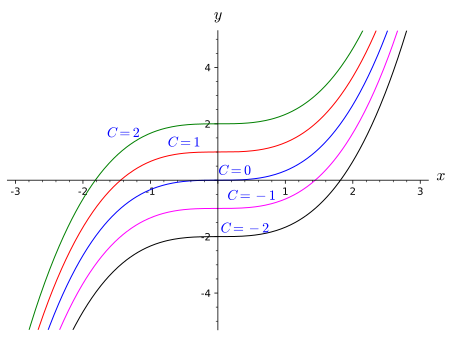
\includegraphics[width=\linewidth]{images/sageplot-primitivas.pdf}}%
%{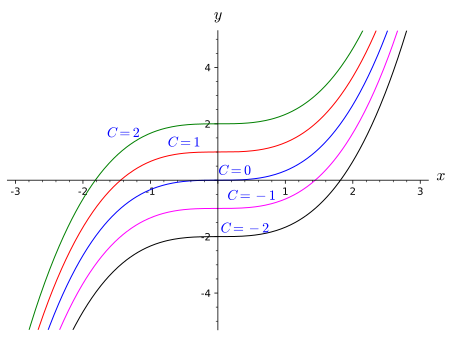
\includegraphics[width=\linewidth]{images/sageplot-primitivas.png}}
\tcblower
\end{figureptx}%
\end{sbspanel}%
\end{sidebyside}%
\footnotetext[1]{Deslocamentos verticas e horizontais do gráfico de uma função conhecida.\label{g:fn:idp63}}%
\begin{example}{}{x:example:ex1-curvas-integrais}%
\begin{enumerate}[font=\bfseries,label=(\alph*),ref=\alph*]
\item{}Encontre a equação da curva integral, \(y=y(x)\), da função \(f(x)=x\) que passe pelo ponto \((2,1)\).%
 \item{}Encontre a equação da curva integral, \(y=y(x)\),  da função \(f(x)=x^2\) que passe pelo ponto \((2,1)\).%
\end{enumerate}
%
\end{example}
\begin{inlineexercise}{}{g:exercise:idp64}%
Encontre a equação da curva integral, \(y=y(x)\),  da função \(f(x)=2x-2\) que passe pelo ponto \((1,2)\).%
\par\smallskip%
\noindent\textbf{\blocktitlefont Dica}.\hypertarget{g:hint:idp65}{}\quad{}Revise \hyperref[x:example:ex1-curvas-integrais]{Exemplo~{\xreffont\ref{x:example:ex1-curvas-integrais}}}.%
\par\smallskip%
\noindent\textbf{\blocktitlefont Resposta}.\hypertarget{g:answer:idp66}{}\quad{}\(y=x^2-2x+3\).%
\end{inlineexercise}
\end{subsectionptx}
%
%
\typeout{************************************************}
\typeout{Subseção 2.2 Integral e Equações diferenciais}
\typeout{************************************************}
%
\begin{subsectionptx}{Integral e Equações diferenciais}{}{Integral e Equações diferenciais}{}{}{x:subsection:subsec-integral-ed}
Uma \terminology{equação diferencial}  é uma igualdade matemática que envolve   derivadas e uma função desconhecida \(y(x)\). Por exemplo, a igualdade%
\begin{gather*}
\frac{\dd y}{\dd x} = x^2 
\end{gather*}
é uma equação diferencial. Nesse caso, a função desconhecida \(y(x)\) pode ser encontrada usando a \hyperref[x:mrow:eq-integral-indefinida]{integral indefinida} como a seguir%
\begin{gather*}
y(x) = \integral{x^2}{x}=\frac{1}{3}x^3 +C.
\end{gather*}
Portanto, dizemos a função \(y(x)=\frac{1}{3}x^3 +C\) é uma \terminology{solução geral} da equação diferencial \(\frac{\dd y}{\dd x} = x^2\). De forma geral, dada uma função conhecida \(f(x)\) a igualdade \begin{assemblage}{}{x:assemblage:assemblage-eq-diferencial}%
%
\begin{gather}
\frac{\dd y}{\dd x} = f(x)\label{x:mrow:eq-diferencial}
\end{gather}
%
\end{assemblage}
 é uma denominada \terminology{equação diferencial} e resolvê-la significa encontrar a função \(y(x)\) que  satisfaça \hyperref[x:mrow:eq-diferencial]{({\xreffont\ref{x:mrow:eq-diferencial}})}. Isto é, obter a \hyperref[x:definition:def-primitiva]{primitiva} de \(f(x)\). Mais diretamente, a solução geral da equação diferencial \hyperref[x:mrow:eq-diferencial]{({\xreffont\ref{x:mrow:eq-diferencial}})} é dada por%
\begin{assemblage}{}{x:assemblage:asse-sol-eq-diferencial}%
%
\begin{gather}
y(x)=\integral{f(x)}{x}\text{.}\label{g:mrow:idp67}
\end{gather}
%
\end{assemblage}
\begin{example}{}{x:example:ex-diferencial-1}%
Encontre a solução geral da equação diferencial  \(\frac{\dd y}{\dd x} = \cos{x}\).%
\par\smallskip%
\noindent\textbf{\blocktitlefont Solução}.\hypertarget{g:solution:idp68}{}\quad{}Já que \(\sin{x}\) é uma primitiva de \(\cos{x}\), a solução para a equação diferencial é%
\begin{equation*}
y(x) = \sin{x} + C.
\end{equation*}
%
\end{example}
\begin{example}{}{x:example:ex-diferencial-2}%
Resolva a equação diferencial \(\frac{\dd y}{\dd x} = 2 + \sin{x}\).%
\par\smallskip%
\noindent\textbf{\blocktitlefont Solução}.\hypertarget{g:solution:idp69}{}\quad{}Resolver a equação diferencial \(\frac{\dd y}{\dd x} = 2 + \sin{x}\) é equivalente a econcontrar a integral%
\begin{align*}
y(x) \amp = \integral{\left(2+ \sin{x}\right)}{x} \amp \quad \hyperref[x:assemblage:asse-sol-eq-diferencial]{\text{Fórmula da solução geral}} \\
\amp =\integral{2}{x} + \integral{\sin{x}}{x}\\
\amp = 2x -\cos{x} + C\text{.}
\end{align*}
%
\end{example}
\begin{inlineexercise}{}{x:exercise:exer1-sol-geral}%
Encontre a solução geral da equação \(\frac{\dd y}{\dd t}=10e^t\).%
\par\smallskip%
\noindent\textbf{\blocktitlefont Dica}.\hypertarget{g:hint:idp70}{}\quad{}Revise \hyperref[x:example:ex-diferencial-2]{Exemplo~{\xreffont\ref{x:example:ex-diferencial-2}}}.%
\par\smallskip%
\noindent\textbf{\blocktitlefont Resposta}.\hypertarget{g:answer:idp71}{}\quad{}\(y(t)= 10e^t + C\).%
\end{inlineexercise}
Frequentemente estamos interssados em encontrar uma única solução para a  equação diferencial. Por exemplo, no \hyperref[x:example:ex1-curvas-integrais]{Exemplo~{\xreffont\ref{x:example:ex1-curvas-integrais}}} encontramaos a equação da para uma \hyperref[x:definition:curvas-integrais]{curva integral} que passa por \((2,1)\). O Problema de encontrar uma função    \(y(x)\), que satisfaça \hyperref[x:mrow:eq-diferencial]{({\xreffont\ref{x:mrow:eq-diferencial}})} e cuja curva integral passa pelo ponto \((x_0,y_0)\)  é denominado    \terminology{problema de valor inicial} e geralmente apresentado da forma \begin{assemblage}{}{x:assemblage:assemblage-}%
%
\begin{gather}
\frac{\dd y}{\dd x}=f(x), \qquad y(x_0)=y_0\label{x:mrow:eq-pvi}
\end{gather}
%
\end{assemblage}
%
\begin{example}{}{x:example:ex1-pvi}%
Resolva o seguinte problema de valor inicial%
\begin{gather*}
\frac{\dd y}{\dd x}=\cos{x}, \qquad y(0)=0 \text{.}
\end{gather*}
%
\par\smallskip%
\noindent\textbf{\blocktitlefont Solução}.\hypertarget{g:solution:idp72}{}\quad{}No \hyperref[x:example:ex-diferencial-1]{Exemplo~{\xreffont\ref{x:example:ex-diferencial-1}}} encontramos a solução geral \(y(x)=\sin{x}+C\) da equação diferencial \(\frac{\dd y}{\dd x}=\cos{x}\). Para resolver o problema de valor inicial deve-se obter o valor de \(C\) para que \(y(0)=0\). Nota-se que \(C=0\), pois%
\begin{equation*}
y(0)=\sin{0} + C=0\text{.}
\end{equation*}
Logo, a curva integral procurada é%
\begin{equation*}
y(x)=\sin{x}\text{.}
\end{equation*}
%
\end{example}
\begin{example}{}{x:example:ex2-pvi}%
Resolva o seguinte problema de valor inicial%
\begin{gather*}
\frac{\dd y}{\dd x}= 2+ \sin{x} \qquad y(3)=5 \text{.}
\end{gather*}
%
\par\smallskip%
\noindent\textbf{\blocktitlefont Solução}.\hypertarget{g:solution:idp73}{}\quad{}Sabe-se do \hyperref[x:example:ex-diferencial-2]{Exemplo~{\xreffont\ref{x:example:ex-diferencial-2}}} que a solução geral \(y(x)=2x - \cos{x} +C\) da equação diferencial \(\frac{\dd y}{\dd x}= 2+ \sin{x}\). Como a curva deve satisfazer \(y(3)=5\), obtemos%
\begin{equation*}
y(3)=2\cdot 3-\cos{3} + C=5
\end{equation*}
de modo que \(C\) vale%
\begin{equation*}
C = 5+\cos{3}-6 \approx -1.99 \quad \color{gray}{\text{calculadora científica}}\text{.}
\end{equation*}
Portanto a solução é%
\begin{equation*}
y(x)= 2x - \cos{x} - 1.99\text{.}
\end{equation*}
\begin{figureptx}{Curva integral \(y(x)= 2x - \cos{x} - 1.99\) que passa pelo ponto \((3,5)\).}{x:figure:fig-pvi2}{}%
\begin{image}{0.25}{0.5}{0.25}%
\IfFileExists{images/curva-integra-pvi2.pdf}%
{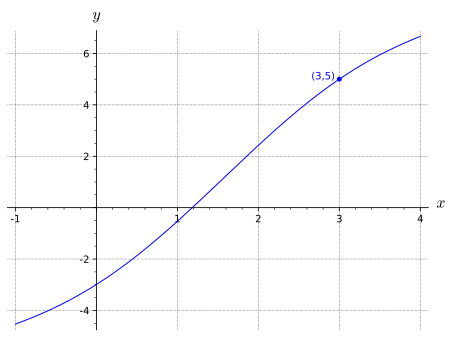
\includegraphics[width=\linewidth]{images/curva-integra-pvi2.pdf}}%
{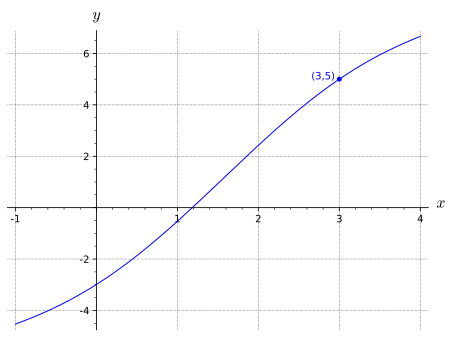
\includegraphics[width=\linewidth]{images/curva-integra-pvi2.png}}
\end{image}%
\tcblower
\end{figureptx}%
%
\end{example}
\begin{inlineexercise}{}{x:exercise:exer-pvi-1}%
\begin{enumerate}[font=\bfseries,label=(\alph*),ref=\alph*]
\item{}Encontre a solução do problema de valor inicial%
\begin{equation*}
\frac{\dd y}{\dd t}=10e^t, \quad y(0)=25\text{.}
\end{equation*}
%
\item{}Encontre a solução do problema de valor inicial%
\begin{equation*}
\frac{\dd y}{\dd t} = 2+ \sin{t}, \quad  y(0)=5\text{.}
\end{equation*}
%
\end{enumerate}
\end{inlineexercise}
\end{subsectionptx}
%
%
\typeout{************************************************}
\typeout{Subseção 2.3 Campos de Direções}
\typeout{************************************************}
%
\begin{subsectionptx}{Campos de Direções}{}{Campos de Direções}{}{}{x:subsection:subsec-resolvendo-e-diferenciais}
Sabe-se  a inclinação da reta tangente à curva  \(y=y(x)\) em dado ponto \((x, y)\) é dada por \(\dd y/\dd x\) para cada \(x\). A Equação \hyperref[x:mrow:eq-diferencial]{({\xreffont\ref{x:mrow:eq-diferencial}})} revela que a inclinação das retas tangentes às curvas integrais de \(f\) no ponto \((x_0, y_0)\) é exatamente  \(f(x_0)\). Com isso é possível entender as "direções" das curvas integrais plotando pequanas porções de suas retas tangentes em cada ponto \((x,y)\)  de uma região retangular. Como resultado teremos o que denominamos de \terminology{campo de direções}. Na \hyperref[x:figure:fig-campo-direcoes]{Figura~{\xreffont\ref{x:figure:fig-campo-direcoes}}\textendash{}{\xreffont\ref{x:figure:fig-campo-direcoes-curva}}} podemos observar que  mesmo não conhecendo a curva integral é possível ter a pespectiva geometrica do seu gráfico.%
\begin{sidebyside}{2}{0.01}{0.01}{0.02}%
\begin{sbspanel}{0.48}[center]%
\begin{figureptx}{Campo de direções das curvas integrais de \(f(x)=x^2\).}{x:figure:fig-campo-direcoes}{}%
\IfFileExists{images/sageplot-campo-direcoes.pdf}%
{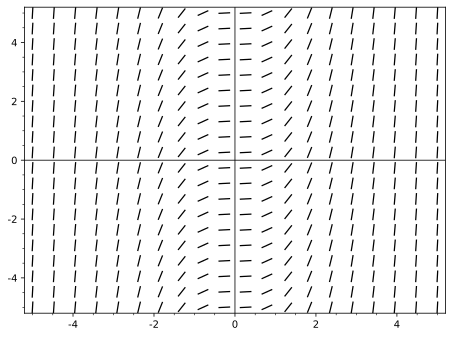
\includegraphics[width=\linewidth]{images/sageplot-campo-direcoes.pdf}}%
{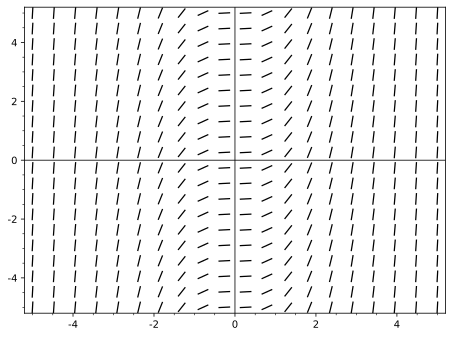
\includegraphics[width=\linewidth]{images/sageplot-campo-direcoes.png}}
\tcblower
\end{figureptx}%
\end{sbspanel}%
\begin{sbspanel}{0.48}[center]%
\begin{figureptx}{Campo de direções e as curvas integrais da função \(f(x)=x^2\).}{x:figure:fig-campo-direcoes-curva}{}%
\IfFileExists{images/sageplot-campo-direcoes-curva.pdf}%
{\includegraphics[width=\linewidth]{images/sageplot-campo-direcoes-curva.pdf}}%
{\includegraphics[width=\linewidth]{images/sageplot-campo-direcoes-curva.png}}
\tcblower
\end{figureptx}%
\end{sbspanel}%
\end{sidebyside}%
\begin{technology}{Faça você mesmo.}{g:technology:idp74}%
\begin{figureptx}{Curvas integrais e campos de direções}{x:figure:figure-interactive-numerical-integral}{}%
\centering
\setlength{\qrsize}{9em}
\setlength{\previewwidth}{\linewidth}
\addtolength{\previewwidth}{-\qrsize}
\begin{tcbraster}[raster columns=2, raster column skip=1pt, raster halign=center, raster force size=false, raster left skip=0pt, raster right skip=0pt]%
\begin{tcolorbox}[previewstyle, width=\previewwidth]%
\IfFileExists{images/interactive-numerical-integral-preview.png}%
{\includegraphics[width=0.80\linewidth,height=\qrsize,keepaspectratio]{images/interactive-numerical-integral-preview.png}}%
{\small{}Specify static image with \mono{@preview} attribute,\\Or create and provide automatic screenshot as \mono{images/interactive-numerical-integral-preview.png} via the \mono{mbx} script}%
\end{tcolorbox}%
\begin{tcolorbox}[qrstyle]%
{\hypersetup{urlcolor=black}\qrcode[height=\qrsize]{/interactive-numerical-integral.html}}%
\end{tcolorbox}%
\end{tcbraster}%
\tcblower
\end{figureptx}%
\end{technology}
\end{subsectionptx}
%
%
\typeout{************************************************}
\typeout{Exercícios 2.4 Exercícios}
\typeout{************************************************}
%
\begin{exercises-subsection}{Exercícios}{}{Exercícios}{}{}{x:exercises:exercises-eq-diferencial}
\par\medskip\noindent%
%
Determine a função \(y=y(x)\), \(x\in\mathbb{R}\), para cada condição dada.%
\begin{exercisegroup}
\begin{divisionexerciseeg}{1}{}{}{g:exercise:idp75}%
\(\frac{\dd y}{\dd x}=3x-1\quad \text{e} \quad y(0)=2\)\end{divisionexerciseeg}%
\begin{divisionexerciseeg}{2}{}{}{g:exercise:idp76}%
\(\frac{\dd y}{\dd x}=\cos{x} \quad \text{e} \quad y(0)=0\)\end{divisionexerciseeg}%
\begin{divisionexerciseeg}{3}{}{}{g:exercise:idp77}%
\(\frac{\dd y}{\dd x}=x^3-x+1 \quad \text{e}\quad  y(1)=1\)\end{divisionexerciseeg}%
\begin{divisionexerciseeg}{4}{}{}{g:exercise:idp78}%
\(\frac{\dd y}{\dd x}=e^{-x} \quad \text{e}\quad  y(0)=1\)\end{divisionexerciseeg}%
\begin{divisionexerciseeg}{5}{}{}{g:exercise:idp79}%
\(\frac{\dd y}{\dd x}=\frac{1}{x^2}\quad  \text{e}\quad  y(1)=1\quad (x>0)\)\end{divisionexerciseeg}%
\begin{divisionexerciseeg}{6}{}{}{g:exercise:idp80}%
\(\frac{\dd y}{\dd x}=3 + \frac{1}{x}\quad  \text{e}\quad  y(1)=2\quad(x>0)\)\end{divisionexerciseeg}%
\end{exercisegroup}
\par\medskip\noindent
\begin{divisionexercise}{7}{}{}{g:exercise:idp81}%
Encontre uma função \(F\) tal que \(F(x) = x + \cos{x}\) e, além disso, \(F (0) = 1\) e \(F'(0) = 2\).%
\end{divisionexercise}%
\begin{divisionexercise}{8}{}{}{g:exercise:idp82}%
Mostre que \(y=xe^{-x} + 2\) é uma solução do problema de valor inicial%
%
\begin{equation*}
\frac{\dd y}{\dd x} = (1-x)e^{-x}, \quad y(0)=2.
\end{equation*}
\end{divisionexercise}%
\par\medskip\noindent%
%
Encontre uma equação da curva que satisfaz as condições dadas.%
\begin{exercisegroup}
\begin{divisionexerciseeg}{9}{}{}{g:exercise:idp83}%
Em cada ponto \((x, y)\) da curva, a inclinação é \(2x + 1\); a curva passa pelo ponto \((−3, 0)\).%
\end{divisionexerciseeg}%
\begin{divisionexerciseeg}{10}{}{}{g:exercise:idp84}%
Em cada ponto \((x, y)\) da curva, a inclinação é \(−\sin{x} \); a curva passa pelo ponto \((0, 2)\).%
\end{divisionexerciseeg}%
\end{exercisegroup}
\par\medskip\noindent
\par\medskip\noindent%
%
Use um recurso gráfico computacional para gerar um campo de direções de cada equação diferencial:%
\begin{exercisegroup}
\begin{divisionexerciseeg}{11}{}{}{g:exercise:idp85}%
\(\frac{\dd y}{\dd x} = x\) na região \(−5 \leq x \leq 5\) e \(−5 \leq y \leq 5.\)%
\end{divisionexerciseeg}%
\begin{divisionexerciseeg}{12}{}{}{g:exercise:idp86}%
\(\frac{\dd y}{\dd x} = \sin{x}\) na região \(−6 \leq x \leq 6\) e \(−6 \leq y \leq 6.\)%
\end{divisionexerciseeg}%
\begin{divisionexerciseeg}{13}{}{}{g:exercise:idp87}%
\(\frac{\dd y}{\dd x} = e^x\) na região \(−6 \leq x \leq 6\) e \(−2 \leq y \leq 2\)%
\end{divisionexerciseeg}%
\end{exercisegroup}
\par\medskip\noindent
\end{exercises-subsection}
\end{sectionptx}
\end{document}